\documentclass[a4paper, 12pt]{article}


%Абзацный отступ

\usepackage{indentfirst}

\usepackage{tablefootnote}  % Cноски для таблиц

%Рисунки

\usepackage{graphicx}
\usepackage{wrapfig}

%Гиперссылки и работа с цветом

\usepackage{hyperref}
\usepackage[rgb]{xcolor}
\hypersetup{			%Гиперссылки
	colorlinks=true, 	%false: ссылки в рамках
	urlcolor=blue		%на URL
}

%Русский язык

\usepackage[T2A]{fontenc}		%кодировка
\usepackage[utf8]{inputenc}		%кодировка исходного текста
\usepackage[english, russian]{babel}	%локализация и переносы


%Математика

\usepackage{amsmath, amsfonts, amssymb, amsthm, mathtools, mathrsfs}

\author{Штрайх Роберт}
\title{Работа 3.3.4. Эффект Холла в полупроводниках}
\date{28 сентября 2021 г.}

\begin{document}
\begin{titlepage}
	\centering
	\vspace{5cm}
	{\scshape\LARGE Московский физико-технический институт \par}
	\vspace{4cm}
	{\scshape\Large Лабораторная работа №3.3.4 \par}
	\vspace{1cm}
	{\huge\bfseries Эффект Холла в полупроводниках \par}
	\vspace{1cm}
	\vfill
\begin{flushright}
	{\Large выполнил студент 006 группы ФЭФМ}\par
	\vspace{0.3cm}
	{\Large Штрайх Роберт}
\end{flushright}
	

	\vfill

% Bottom of the page
	Долгопрудный, 2021 г.
\end{titlepage}

\newpage
\textbf{Цель работы:} измерение подвижности и концентрации носителей заряда в полупроводниках.

\textbf{В работе используются:} электромагнит с регулируемым источником питания; вольтметр; амперметр; миллиамперметр; милливеберметр или миллитесламетр; источник питания (1,5 В), образцы легированного германия.

\section{Теоретическое введение}

Во внешнем магнитном поле \textbf{\textit{B}} на заряды действует сила Лоренца:

\begin{equation} \label{Lorens}
\textbf{\textit{F}} = q\textbf{\textit{E}} + q\textbf{\textit{u}} \times \textbf{\textit{B}}.
\end{equation}
Эта сила вызывает движение носителей, направление которого в общем случае не совпадает с \textbf{\textit{E}}. Возникновение поперечного тока электрического поля в образце, помещённом во внешнее магнитное поле, называют \textit{эффектом Холла.}

В работе изучаются особенности проводимости проводников в геометрии \textit{мостика Холла}. Ток пропускается по плоской полупроводниковой пластинке, помещённой в перпендикулярное пластинке магнитное поле. Измеряется разность потенциалов между краями пластинки в поперечном к току направлении. По измерениям определяется \textit{константа Холла}, тип проводимости (\textit{электронный} или \textit{дырочный}) и на основе соотношения \eqref{R_x} вычисляется концентрация основных носителей заряда.

\section{Расчётные формулы}

\begin{itemize}
\item ЭДС Холла:
\begin{equation} \label{E}
\mathscr{E_\text{х}} = U_{34} - U_0,
\end{equation}
\item Постоянная Холла:
\begin{equation} \label{R_x}
R_x = -\frac{\mathscr{E_\text{х}}}{B}\cdot\frac{a}{I} = \frac{1}{nq},
\end{equation}
\item Концентрация носителей тока в образце:
\begin{equation} \label{n}
n = \frac{1}{R_xe},
\end{equation}
\item Удельная проводимость материала образца:
\begin{equation}	\label{sigma}
\sigma = \frac{IL_{35}}{U_{35}al},
\end{equation}
\item Подвижность носителей тока:
\begin{equation}	\label{b}
b = \frac{\sigma}{en}.
\end{equation}
\end{itemize}

\section{Экспериментальная установка}

\begin{figure}[h]
\begin{center}
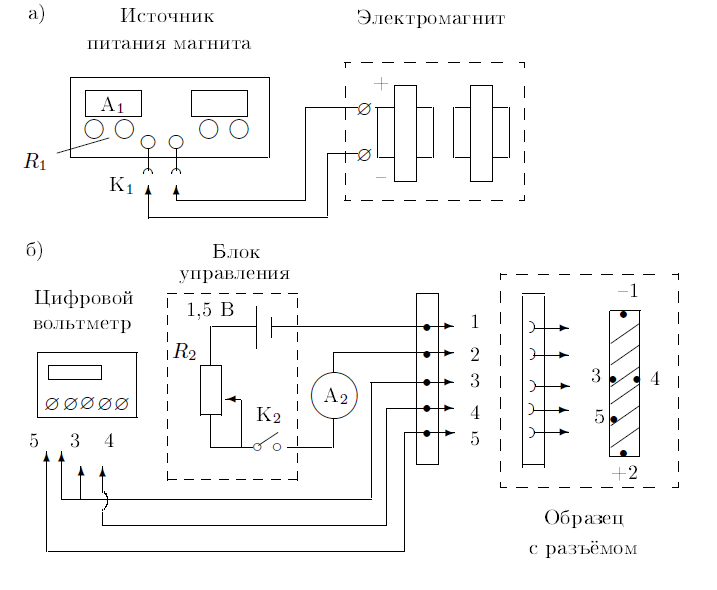
\includegraphics[width=1\textwidth]{Рисунок_установки}
\end{center}
\caption{Схема установки для исследования эффекта Холла в полупроводниках}
\end{figure}

\newpage

\section{Ход работы}

1. Произведём калибровку магнита - определим связь между индукцией $B$ магнитного поля  в зазоре электромагнита и током $I_{м}$ через обмотки магнита. Результаты занесём в таблицу \ref{B(I)tab} и представим на графике \ref{B(I)graph}.

%С РУССКИМИ ИНДЕКСАМИ СТАВЬ {}

\begin{table}[h]	
\caption{Зависимость $B(I_\text{м})$}
\begin{tabular}{|l|l|l|l|l|l|l|l|l|} 	
\hline
\textit{$I_\text{м}$, А}   & 0,15   & 0,30   & 0,46   & 0,60   & 0,75   & 0,90   & 1,05   & 1,28    \\
\hline
\textit{$B$, мТл} & 179,40 & 327,95 & 503,65 & 638,85 & 772,55 & 878,55 & 952,60 & 1033,35 \\
\hline
\end{tabular}
\label{B(I)tab}
\end{table}

2. Проведём измерение ЭДС Холла. Снимем зависимость напряжения $U_{34}$ от тока $I_{м}$ через обмотки магнита (с учётом $U_0$). Выполним серию измерений для различных токов $I$ через образец (от 0,3 до 1 мА). Результаты измерений занесём в таблицу \ref{ЭДС таблица} и построим на их основе семейство прямых $\mathscr{E_\text{х}} = f(B)$ (рис. \ref{E(B)graph}).


\begin{table}[h]
\caption{Зависимость $\mathscr{E_\text{x}}(B)$}
\small
\begin{tabular}{|l|l|l|l|l|l|l|l|l|l|}
\hline
\textit{B, мТл}  &  & 179,40 & 327,95 & 503,65 & 638,85 & 772,55 & 878,55 & 952,60 & 1033,35 \\ \hline
\textit{$I_{м}$, А}   & \textbf{}          & 0,15   & 0,30   & 0,46   & 0,60   & 0,75   & 0,90   & 1,05   & 1,28    \\ \hline
\textit{$U_{34}$, мВ} & \textit{$I=0,3$ мА}  & -0,100 & -0,150 & -0,193 & -0,235 & -0,270 & -0,302 & -0,325 & -0,347  \\ \cline{1-1} \cline{3-10} 
$\mathscr{E_\text{х}}$, \textit{мВ}   &  & -0,157 & -0,207 & -0,250 & -0,292 & -0,327 & -0,359 & -0,382 & -0,404  \\ \hline
\textit{$U_{34}$, мВ} & \textit{$I=0,4$ мА}  & -0,143 & -0,197 & -0,261 & -0,315 & -0,363 & -0,403 & -0,432 & -0,463  \\ \cline{1-1} \cline{3-10} 
$\mathscr{E_\text{х}}$, \textit{мВ}   &  & -0,230 & -0,284 & -0,348 & -0,402 & -0,450 & -0,490 & -0,519 & -0,550  \\ \hline
\textit{$U_{34}$, мВ} & \textit{$I=0,5$ мА}  & -0,118 & -0,251 & -0,321 & -0,392 & -0,453 & -0,501 & -0,540 & -0,575  \\ \cline{1-1} \cline{3-10} 
$\mathscr{E_\text{х}}$, \textit{мВ}   &          & -0,226 & -0,359 & -0,429 & -0,500 & -0,561 & -0,609 & -0,648 & -0,683  \\ \hline
\textit{$U_{34}$, мВ} & \textit{$I=0,6$ мА}  & -0,212 & -0,297 & -0,387 & -0,468 & -0,547 & -0,604 & -0,647 & -0,689  \\ \cline{1-1} \cline{3-10} 
$\mathscr{E_\text{х}}$, \textit{мВ}   &  & -0,343 & -0,428 & -0,518 & -0,599 & -0,678 & -0,735 & -0,778 & -0,820  \\ \hline
\textit{$U_{34}$, мВ} & \textit{$I=0,7$ мА}  & -0,251 & -0,354 & -0,455 & -0,549 & -0,637 & -0,705 & -0,759 & -0,808  \\ \cline{1-1} \cline{3-10} 
$\mathscr{E_\text{х}}$, \textit{мВ}   &                    & -0,404 & -0,507 & -0,608 & -0,702 & -0,790 & -0,858 & -0,912 & -0,961  \\ \hline
\textit{$U_{34}$, мВ} & \textit{$I=0,8$ мА}  & -0,282 & -0,402 & -0,522 & -0,627 & -0,725 & -0,807 & -0,866 & -0,921  \\ \cline{1-1} \cline{3-10} 
$\mathscr{E_\text{х}}$, \textit{мВ}   &                    & -0,456 & -0,576 & -0,696 & -0,801 & -0,899 & -0,981 & -1,040 & -1,095  \\ \hline
\textit{$U_{34}$, мВ} & \textit{$I=0,9$ мА}  & -0,322 & -0,454 & -0,578 & -0,703 & -0,817 & -0,905 & -0,973 & -1,035  \\ \cline{1-1} \cline{3-10} 
$\mathscr{E_\text{х}}$, \textit{мВ}   &                    & -0,518 & -0,650 & -0,774 & -0,899 & -1,013 & -1,101 & -1,169 & -1,231  \\ \hline
\textit{$U_{34}$, мВ} & \textit{$I=1,0$ мА}  & -0,353 & -0,500 & -0,647 & -0,788 & -0,907 & -1,008 & -1,078 & -1,149  \\ \cline{1-1} \cline{3-10} 
$\mathscr{E_\text{х}}$, \textit{мВ}   &                    & -0,571 & -0,718 & -0,865 & -1,006 & -1,125 & -1,226 & -1,296 & -1,367  \\ \hline
\textit{$U_{34}$, мВ} & \textit{$I=1,0$ мА\tablefootnote{Здесь поле направлено в обратную сторону}} & -0,047 & 0,101  & 0,245  & 0,384  & 0,503  & 0,597  & 0,676  & 0,741   \\ \cline{1-1} \cline{3-10} 
$\mathscr{E_\text{х}}$, \textit{мВ}   &                    & -0,231 & -0,083 & 0,061  & 0,200  & 0,319  & 0,413  & 0,492  & 0,557   \\ \hline
\end{tabular}
\label{ЭДС таблица}
\end{table}

4. Определим по графику \ref{E(B)graph} угловые коэффициенты прямых и построим график зависимости $k = f(I)$ (рис. \ref{k(I)graph}). По этому графику определим величину постоянной Холла. Погрешность рассчитаем по методу наименьших квадратов, учитывая погрешности приборов:

\[R_\text{х} = -ka = (9,1\pm0,1)\cdot10^{-4} \frac{\text{м}^3}{\text{Кл}},\] 

Относительная погреншность составляет 1,32\text{\%}.

5. Определим знак носителей заряда в образце, зная направление тока в образце, направление магнитного поля и знак ЭДС Холла. Получаем, что проводимость \textbf{дырочная}.

6. Рассчитаем концентрацию $n$ носителей тока:

\[n = \frac{1}{R_\text{х}e} = (6,87\pm0,09)\cdot10^{21} \text{м}^{-3},\]

7. По формуле \ref{sigma} рассчитаем удельную проводимость образца. При $I = $ 1 мА, $U_{35} = -4,065$ мВ; параметры образца: $a = $ 1 мм, $l = $ 4 мм, $L_{35} = $ 5 мм

\[\sigma = (307,5\pm4,1) \text{Ом}\cdot\text{м}^{-1},\]

8. Вычислим по формуле \ref{b} подвижность $b$ носителей тока:

\[b = (2796,4\pm36,9) \frac{\text{см}^2}{\text{В}\cdot\text{с}},\]

Относительная погрешность составляет 1,32\text{\%}.

Табличное значение проводимости:

\[b_{теор} = 3900 \frac{\text{см}^2}{\text{В}\cdot\text{с}}.\]

\section{Выводы}

В ходе работы был исследован эффект Холла в полупроводнике-германии, выявлено, что в нём преобладает дырочная проводимость. Были вычислены такие величины, как постоянная Холла, концентрация носителей тока, удельная проводимость образца и подвижность носителей тока:

\[R_\text{х} = (9,1\pm0,1)\cdot10^{-4} \frac{\text{м}^3}{\text{Кл}},\] 

\[\varepsilon_{R_\text{х}} = 1,32 \text{\%}\]

\[n = \frac{1}{R_\text{х}e} = (6,87\pm0,09)\cdot10^{21} \text{м}^{-3},\]

\[\varepsilon_n = 1,2 \text{\%}\]

\[\sigma = (307,5\pm4,1) \text{Ом}\cdot\text{м}^{-1},\]

\[\varepsilon_{\sigma} = 1,3 \text{\%}\]

\[b = (2796,4\pm36,9) \frac{\text{см}^2}{\text{В}\cdot\text{с}},\]

\[\varepsilon_b = 1,32 \text{\%}\]

Табличное значение проводимости:

\[b_{теор} = 3900 \frac{\text{см}^2}{\text{В}\cdot\text{с}}.\]

Возможная причина несовпадения табличного и экспериментального значений проводимости в том, что образец является не чистым, а легированным германием.

\newpage

\section{Приложение}

\begin{figure}[h!]
\begin{center}
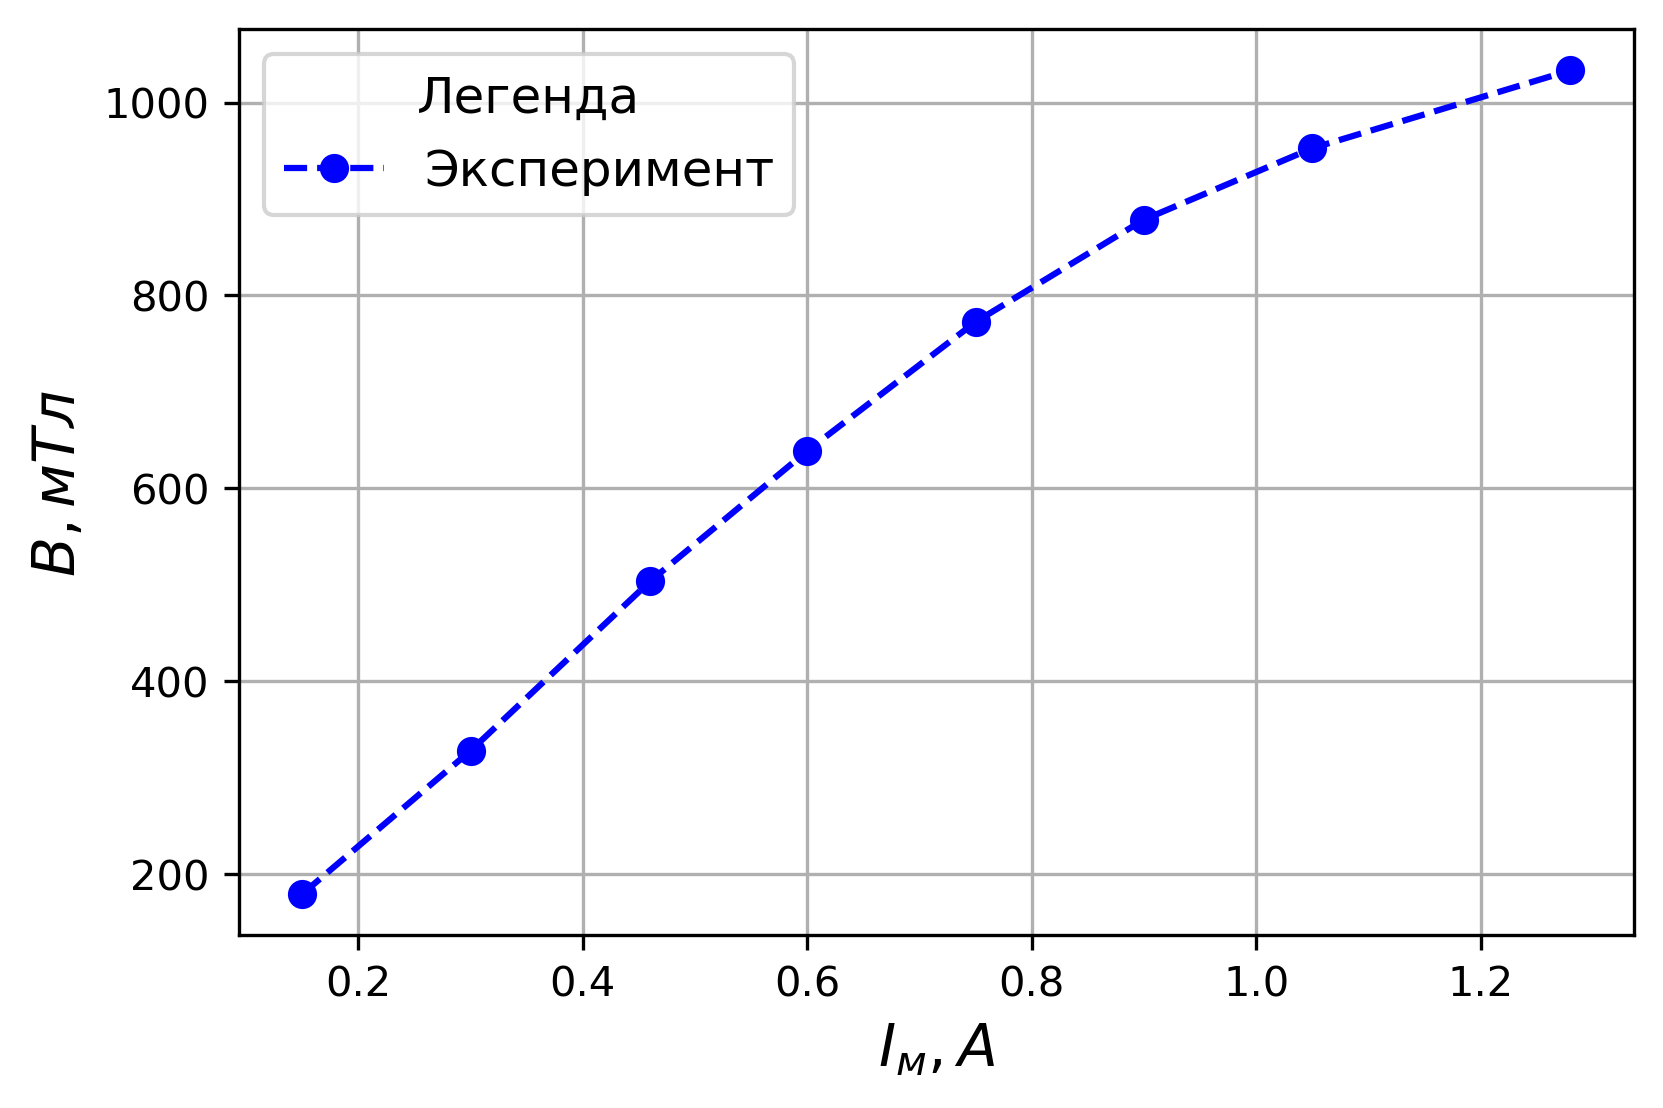
\includegraphics{graphB(I).png}
\end{center}
\caption{График зависимости $B(I_\text{м})$}
\label{B(I)graph}
\end{figure}

\begin{figure}[h!]
\begin{center}
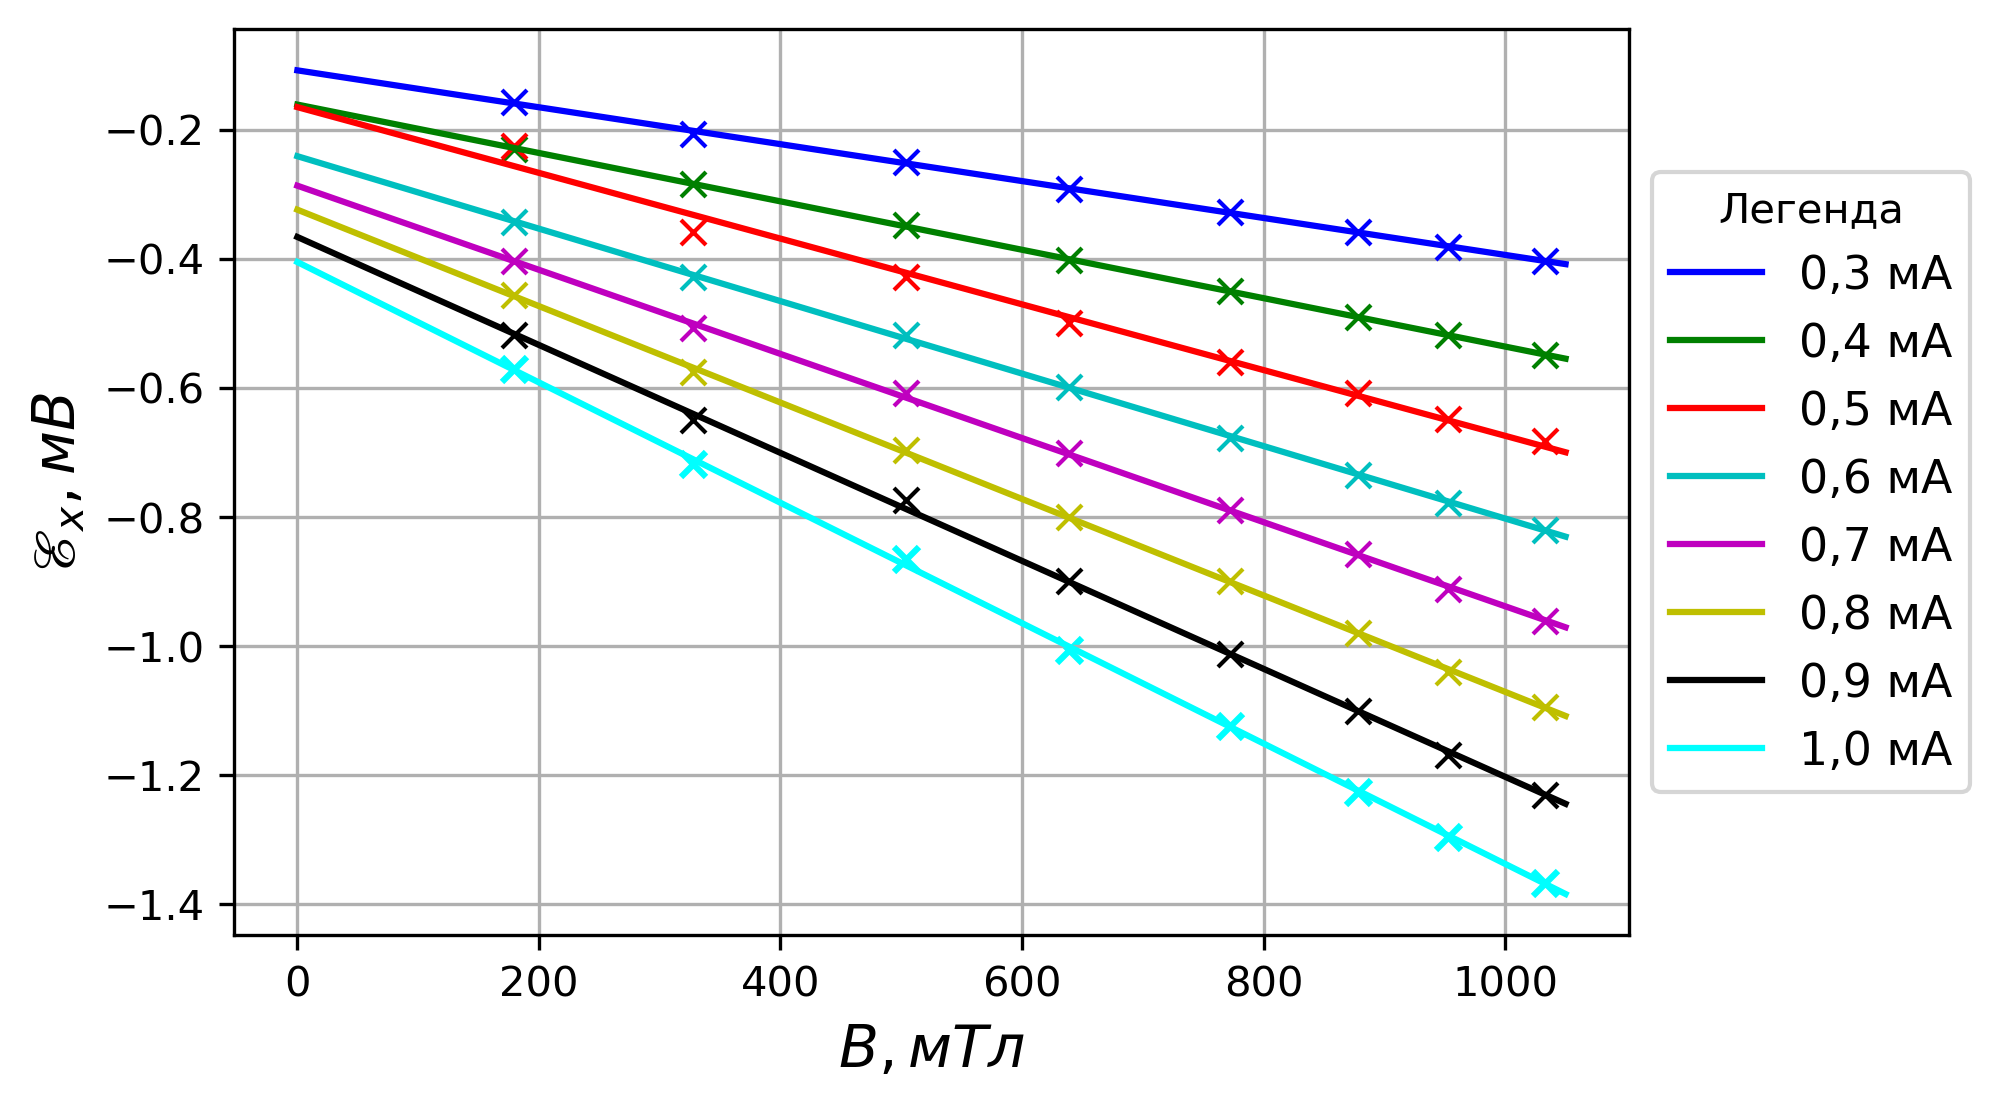
\includegraphics{graphE(B).png}
\end{center}
\caption{Семейство зависимостей $\mathscr{E_\text{x}}(B)$}
\label{E(B)graph}
\end{figure}

\begin{figure}[h!]
\begin{center}
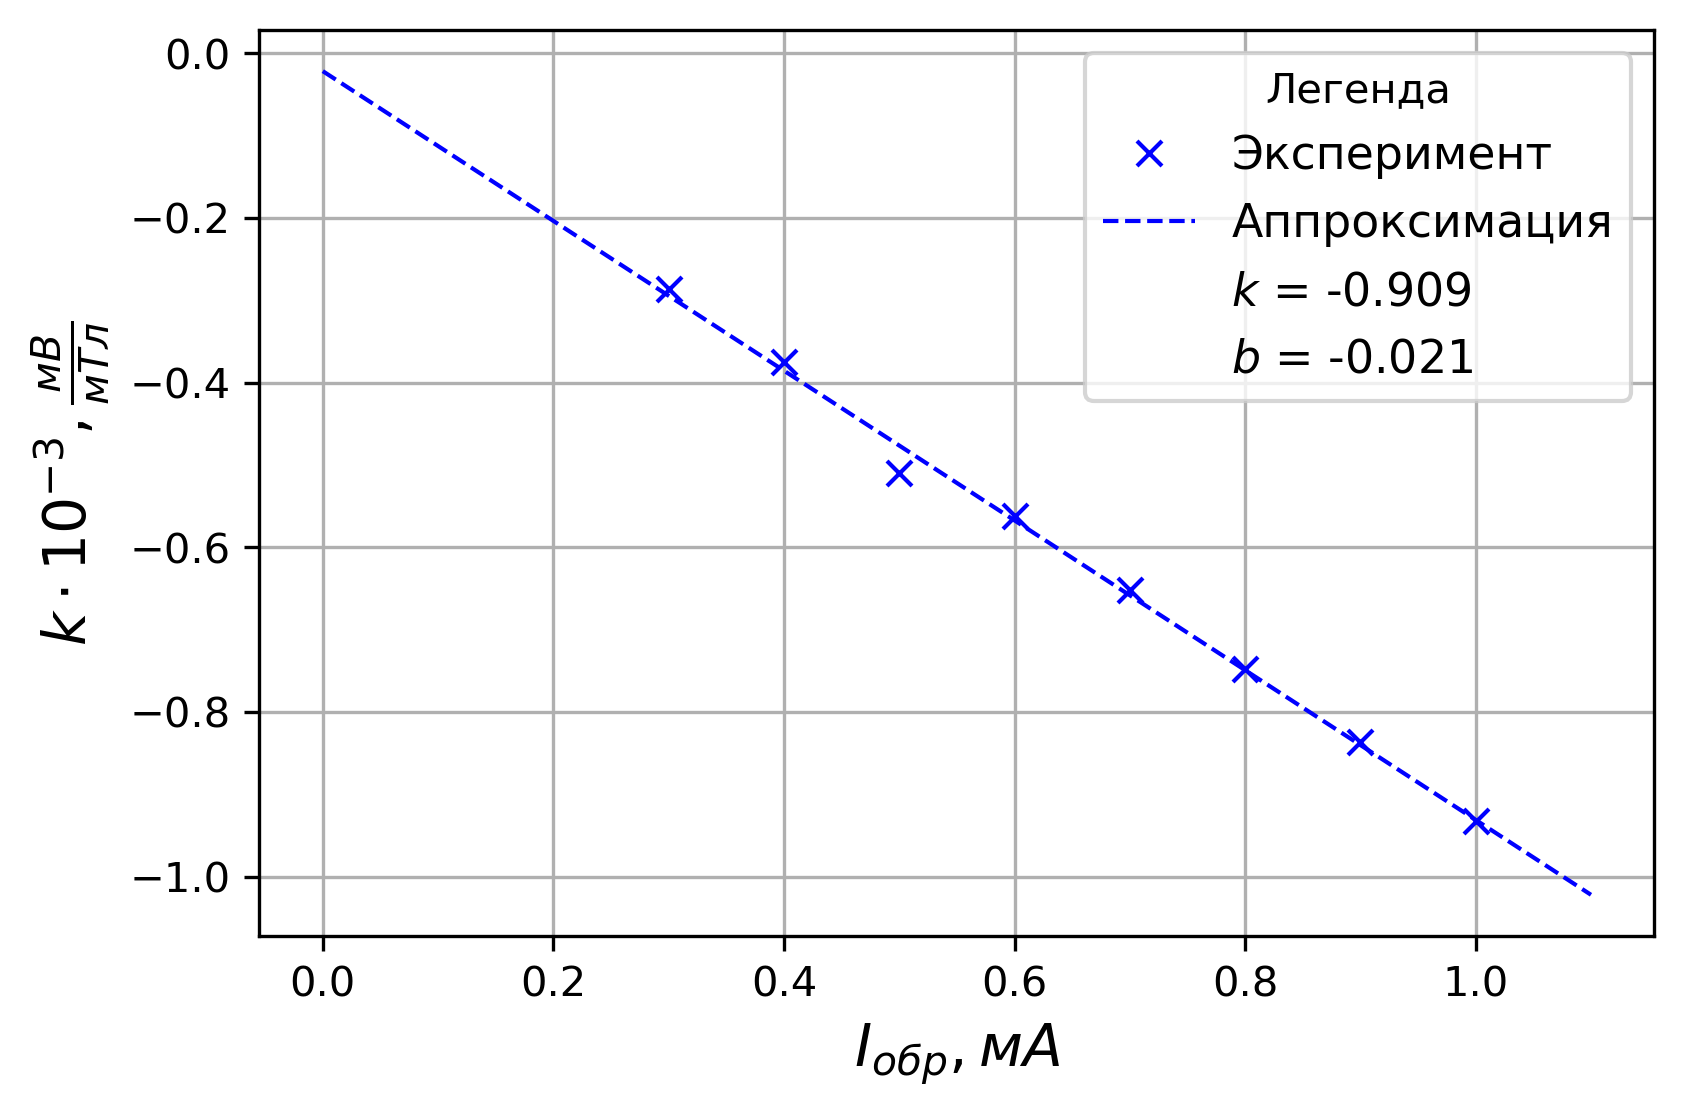
\includegraphics{graphk(I).png}
\end{center}
\caption{График зависимости $k(I)$}
\label{k(I)graph}
\end{figure}

\end{document}

